\documentclass[11pt]{article}
\usepackage[utf8]{inputenc}
\usepackage[T1]{fontenc}
\usepackage{graphicx}
\usepackage[portuguese]{babel}
\usepackage{geometry}
\usepackage{listings}
\usepackage{hyperref}
\usepackage{bookmark}
\usepackage{float}
\graphicspath{ {./img/} }
\begin{document}

\title{Malha aberta}
\maketitle

\section{Modelo de simulação}
\begin{figure}[!h]
\begin{center}
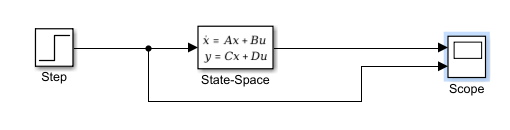
\includegraphics[width=12cm]{modelo.PNG}
\caption{Diagrama de blocos}
\label{fig1.1}
\end{center}
\end{figure}
\begin{figure}[!h]
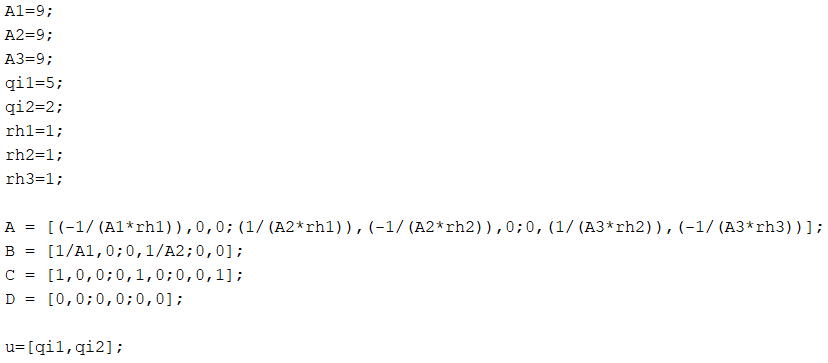
\includegraphics[width=15cm]{params.png}
\caption{Inicialização de parâmetros e matrizes}
\label{fig1.2}
\end{figure}

\pagebreak
\section{Simulações}
Para melhor entendimento do sistema a controlar e como meio de podermos concluir quais as respostas do sistema a mudanças de parâmetros, serão efetuadas algumas simulações.
Inicialmente será testada a resposta do sistema a mudanças de valores das resistências hidráulicas e de seguida a mudanças do valor de área dos 3 tanques, estes que se encontram a 9$m^2$ inicialmente.
Note-se que quaisquer comparações referidas nos comentários de cada simulação, estarão a ser feitas em relação à figura \ref{fig2.1}.
\subsection{Rh1=1$\frac{m}{m^3/s}$, Rh2=1$\frac{m}{m^3/s}$, Rh3=1$\frac{m}{m^3/s}$}
\begin{figure}[!h]
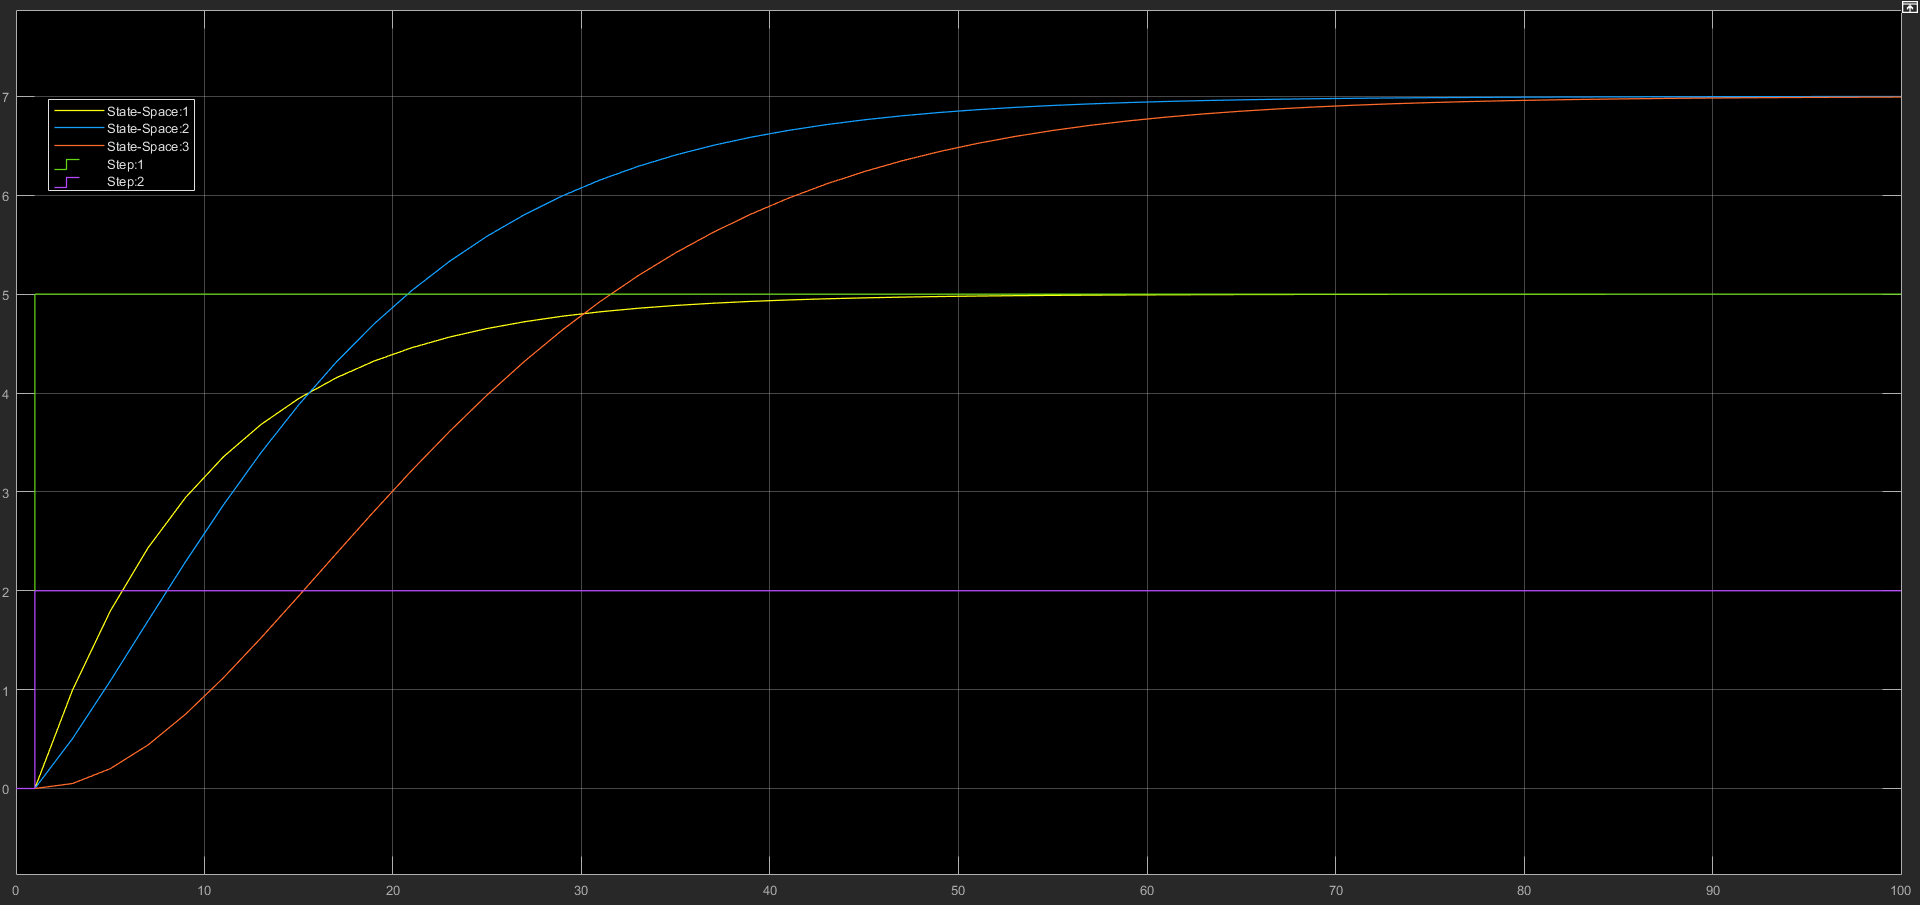
\includegraphics[width=16cm]{initial.png}
\caption{Rh1=1$\frac{m}{m^3/s}$, Rh2=1$\frac{m}{m^3/s}$, Rh3=1$\frac{m}{m^3/s}$}
\label{fig2.1}
\end{figure}
Tendo todas as resistências hidráulicas como valor 1, e sabendo que qi1=5$m^3/s$ e qi2=2$m^3/s$, observa-se que em regime permanente h1 = 5m, h2 = 7m e h3 = 7m. h1 é o primeiro a entrar em regime permanente, seguido de h2, e  por último, h3.
\pagebreak
\subsection{Rh1$\frac{m}{m^3/s}$=2,Rh2$\frac{m}{m^3/s}$=1,Rh3=1$\frac{m}{m^3/s}$}
\begin{figure}[!h]
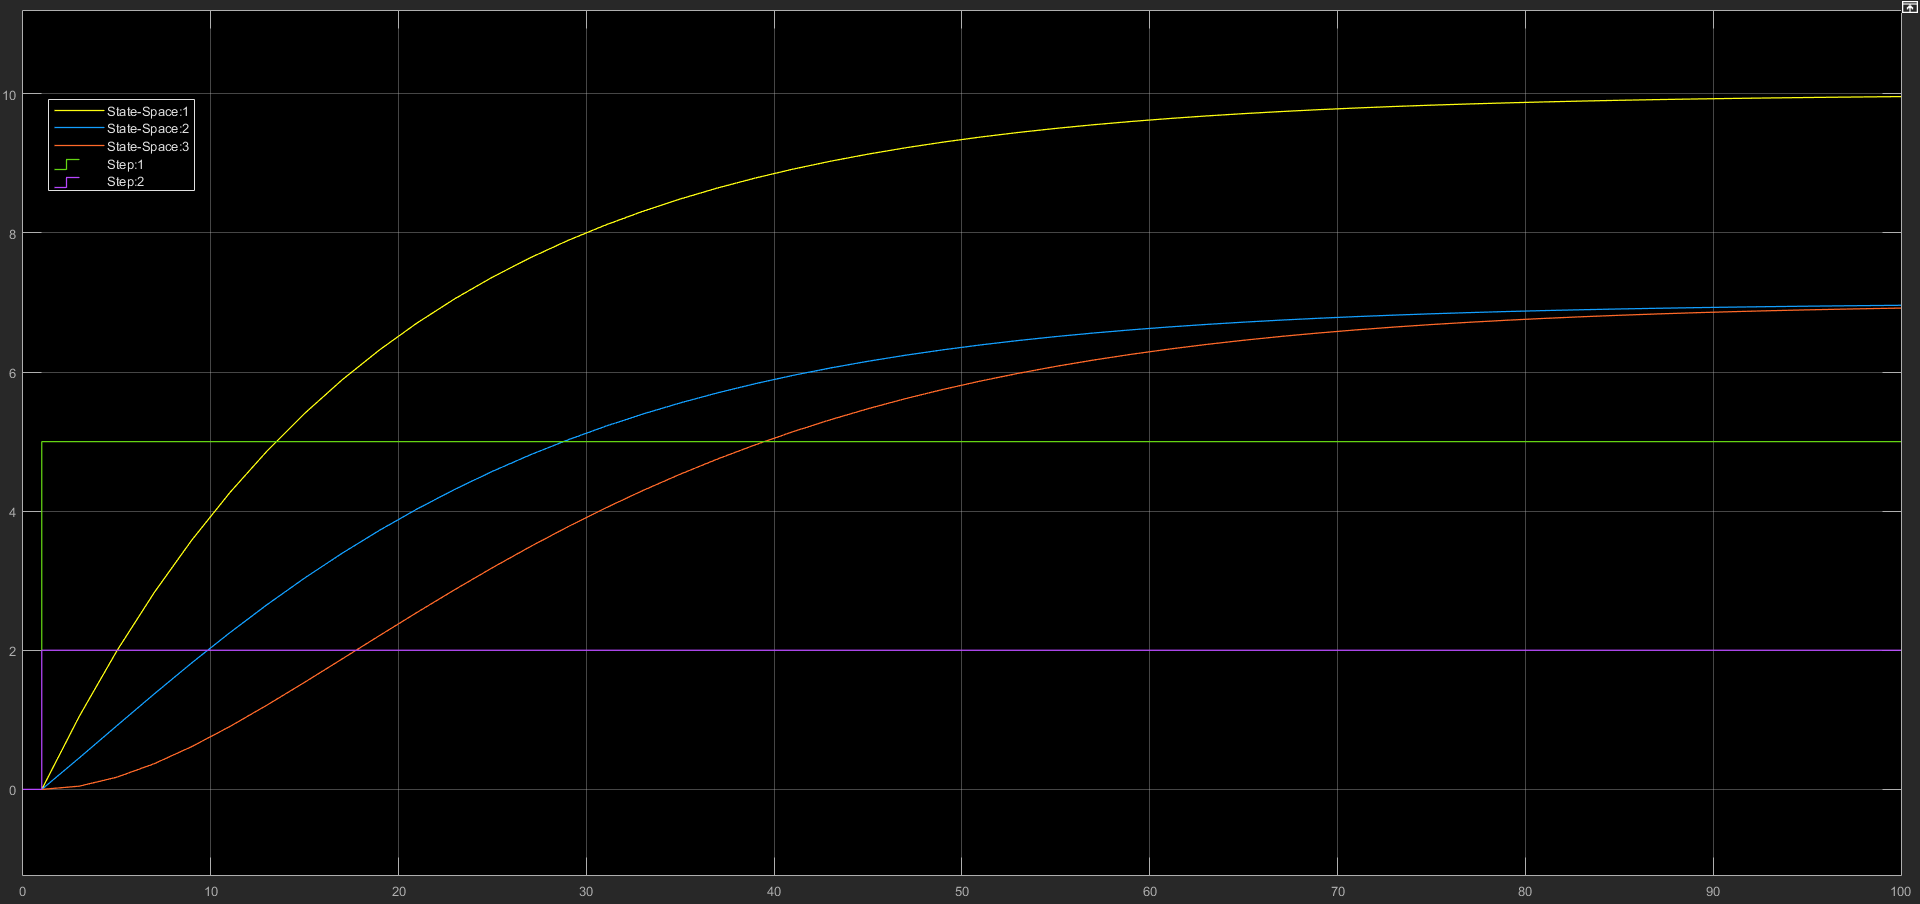
\includegraphics[width=16cm]{rh1.png}
\caption{Rh1=2$\frac{m}{m^3/s}$, Rh2=1$\frac{m}{m^3/s}$, Rh3=1$\frac{m}{m^3/s}$}
\label{fig2.2}
\end{figure}
Alterando apenas o valor de Rh1 para o dobro, verifica-se uma resposta mais lenta do sistema, de forma que todas as variáveis de saída demoram mais tempo a atingir o regime permanente. Verifica-se tembém que o valor em regime permanente h2 e h3 não sofre alteração, mas o valor de h1 passa a ser o dobro, o que faz sentido uma vez que o output de água do tanque 1 passa para metade, logo acumula.
\pagebreak
\subsection{Rh1=1$\frac{m}{m^3/s}$,Rh2=2$\frac{m}{m^3/s}$,Rh3=1$\frac{m}{m^3/s}$}
\begin{figure}[!h]
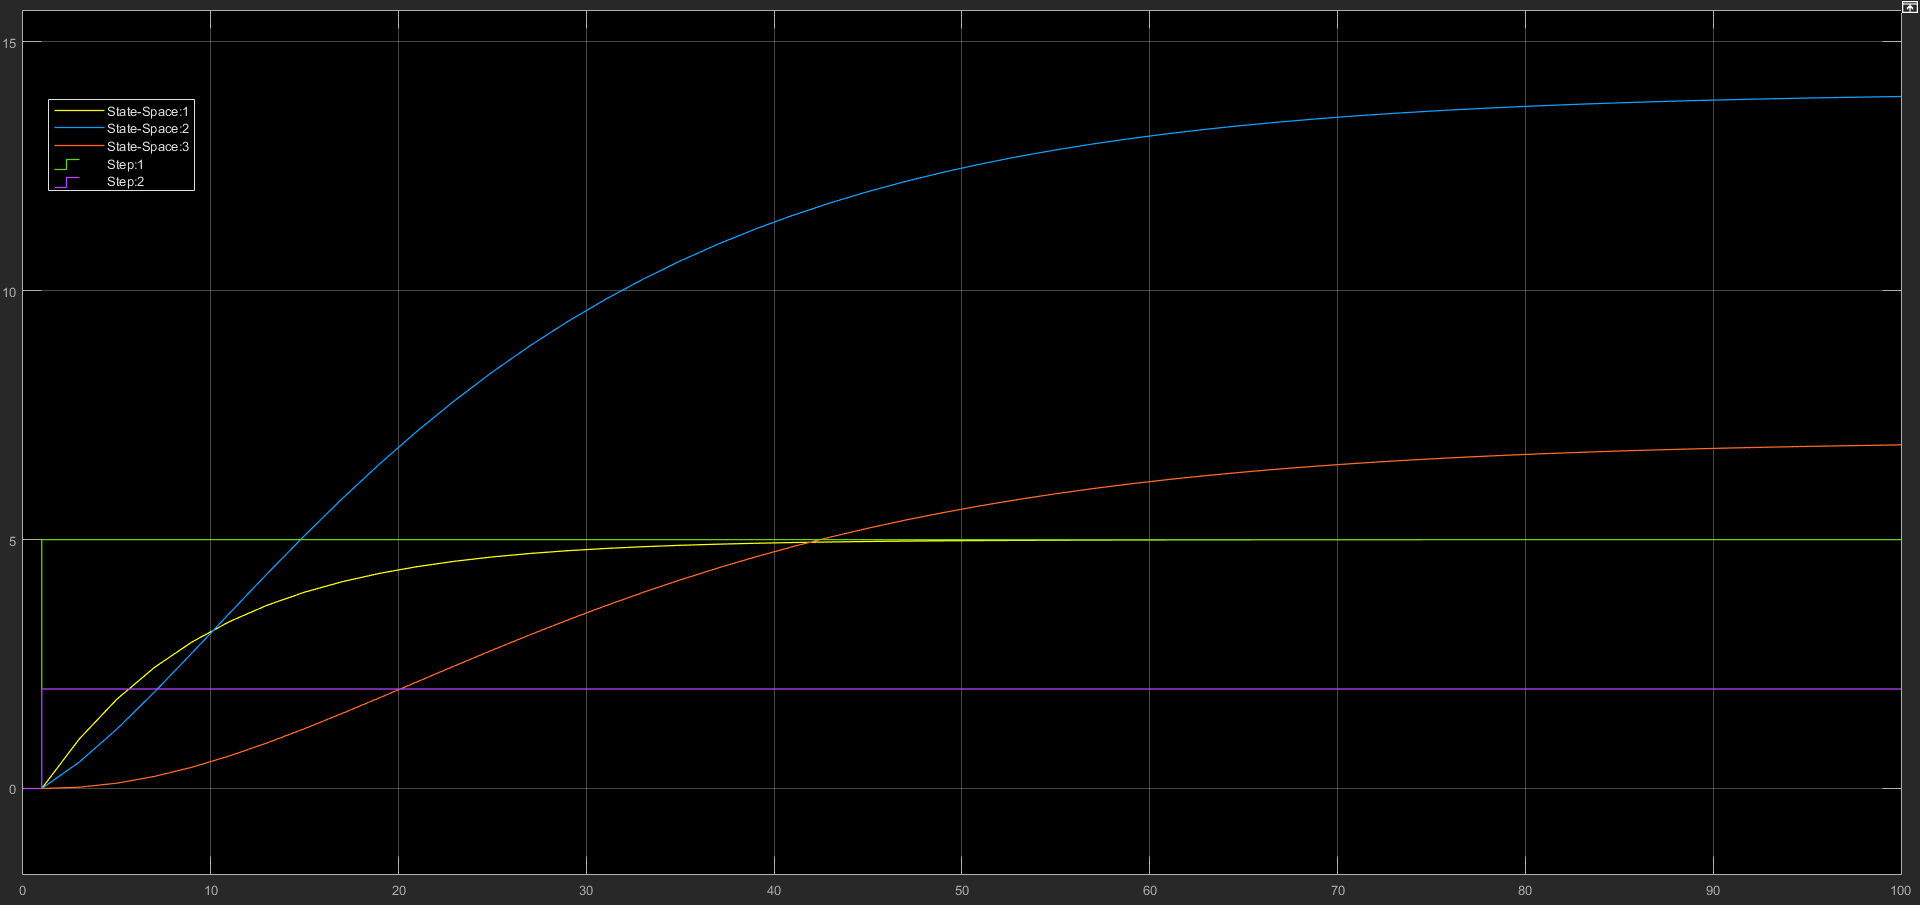
\includegraphics[width=16cm]{rh2.png}
\caption{Rh1=1$\frac{m}{m^3/s}$, Rh2=2$\frac{m}{m^3/s}$, Rh3=1$\frac{m}{m^3/s}$}
\label{fig2.3}
\end{figure}
Repondo o valor de Rh1 a 1 e aumentando agr Rh2 para o dobro, verifica-se que valor de h1 não sofre qualquer alteração em nenhum estado comparativamente com a simulação inicial(\ref{fig2.1}), isto é, não altera ser valor em regime permanente, nem o tempo que demora a atingi-lo. Quanto ao valor de h2 e regime permanente, como previsto, passa para o dobro, demorando também mais tempo para o atingir. O valor em regime permanente de h3 mantém-se ainda em 7m, demorando apenas mais tempo a ser atingido uma vez que o caudal de saída do tanque 2 é menor. 

\pagebreak
\subsection{Rh1=1$\frac{m}{m^3/s}$,Rh2=1$\frac{m}{m^3/s}$,Rh3=2$\frac{m}{m^3/s}$}
\begin{figure}[!h]
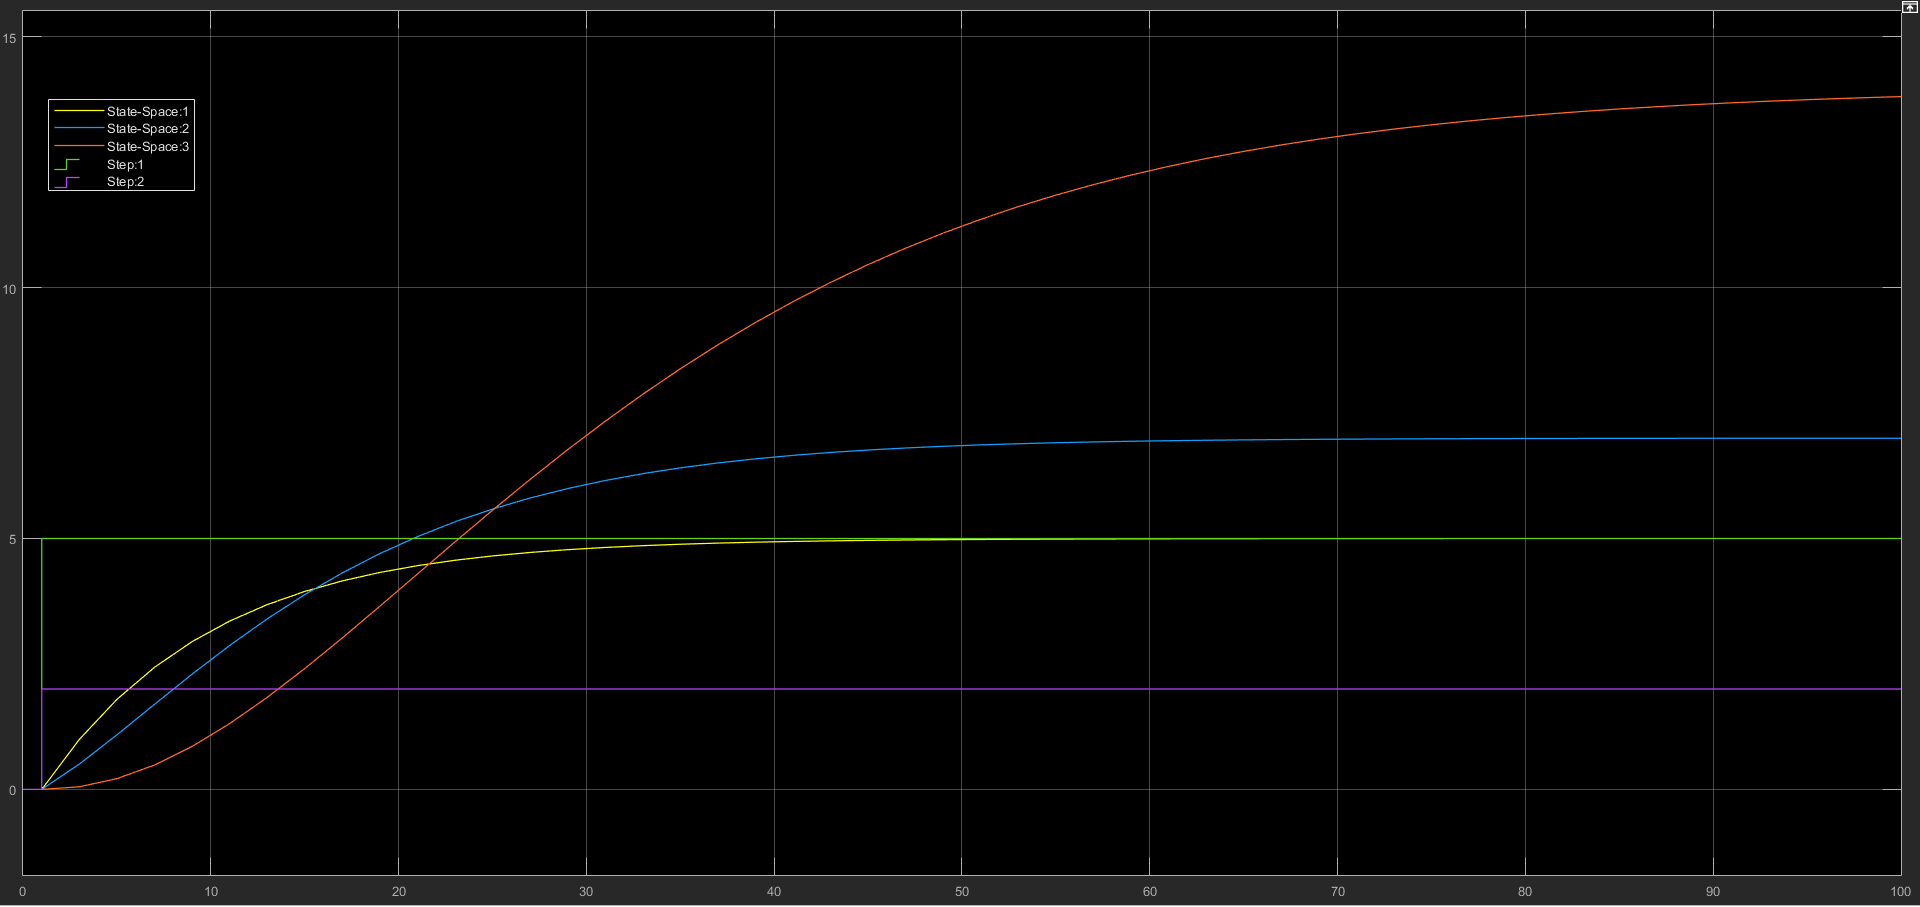
\includegraphics[width=16cm]{rh3.png}
\caption{Rh1=1$\frac{m}{m^3/s}$, Rh2=1$\frac{m}{m^3/s}$, Rh3=2$\frac{m}{m^3/s}$}
\label{fig2.4}
\end{figure}
Com Rh1=1$\frac{m}{m^3/s}$, Rh2=1$\frac{m}{m^3/s}$ e Rh3=2$\frac{m}{m^3/s}$ (dobro), verifica-se que h1 e h2 não sofrem quaisquer alterações em relação à simulação inicial (\ref{fig2.1}). Quanto a h3, como esperado, o seu valor em regime permanente passa para o dobro, visto que a quantidade de água que sai do tanque 3 passa para metade, e o tempo que demora atingir o regime permanente aumenta também visto que o valor que atinge é maior e tem o mesmo caudal à entrada.
\pagebreak
\subsection{Rh1=1$\frac{m}{m^3/s}$,Rh2=1$\frac{m}{m^3/s}$,Rh3=1$\frac{m}{m^3/s}$, Aérea dos 3 tanques=3$m^2$}
\begin{figure}[!h]
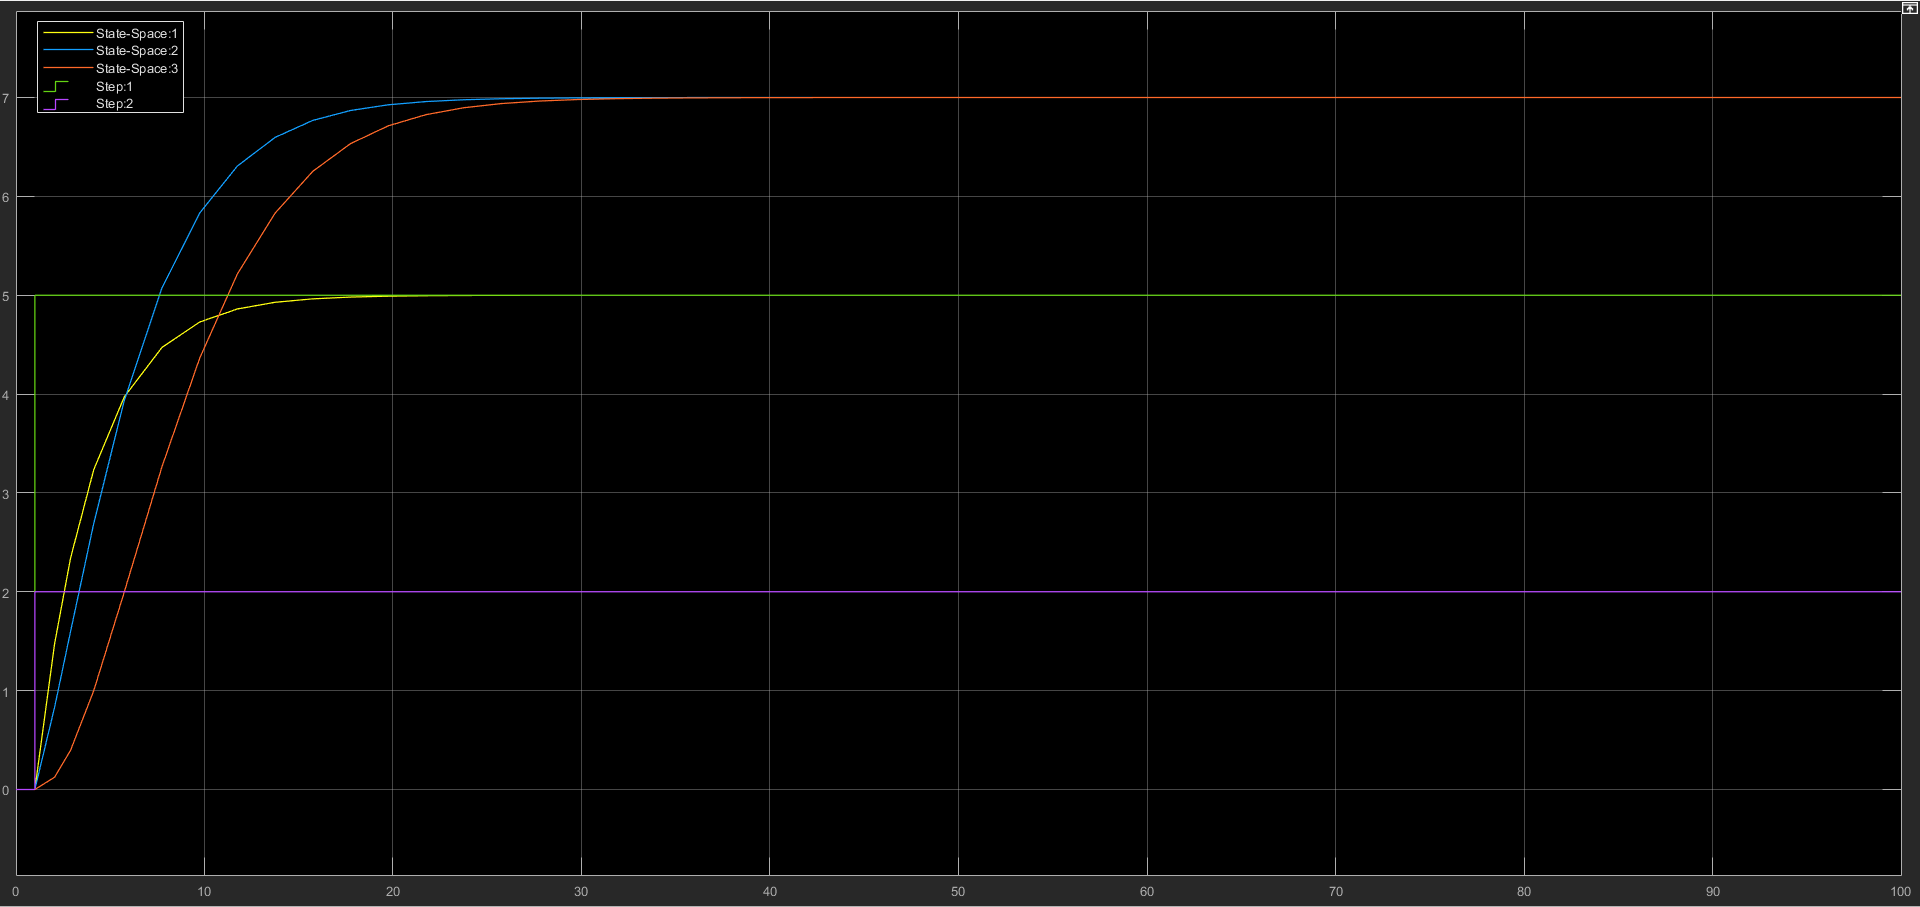
\includegraphics[width=16cm]{A3.png}
\caption{Rh1=1$\frac{m}{m^3/s}$, Rh2=1$\frac{m}{m^3/s}$, Rh3=1$\frac{m}{m^3/s}$, áerea dos tanques=3$m^2$}
\label{fig2.5}
\end{figure}
Alterando apenas o valor da área, verifica-se que não há qualquer alteração nos valores das variáveis em regime permanente, apenas muda o tempo que demora para que estas lá cheguem.
\section{Conclusão}
Com as simulações efetuadas, foi possível tirar algumas conclusões:
\begin{itemize}
\item Alterações nos valores das resistências hidráulicas provoca uma alteração na altura a que a água consegue atingir no/nos tanque/tanques em questão, não alterando o valor em regime permanente das alturas dos restantes tanques;
\item Alterações nos valores das resistências hidráulicas provocam uma resposta mais lenta do sistema, fazendo com que o regime permanente seja atingido mais tarde para todas as alturas dos tanques cuja resistência hidráulica foi alterada, e todos os tanques que se seguirem. Tanques que se encontrarem antes dos que a resistência hidráulica foi alterada não sofrem quaisquer alterações.
\item Alterações nos valores das áreas dos tanques provocam alterações no tempo de resposta do sistema, embora não influenciem os valores em regime permanente.
\end{itemize}

\end{document}
